\section{测试结果}

拿到源代码之后参照第 \ref{runtime} 节\nameref{runtime}进行编译,得到对应平台的二进制可执行文件之后,就可以进行测试了。

首先是在 Windows 平台上,编译之后生成 {\sf huff.exe},在当前目录下键入程序名称 \verb|huff| 即可显示帮助信息,如图 \ref{win_huff}:

\begin{figure}[htp]
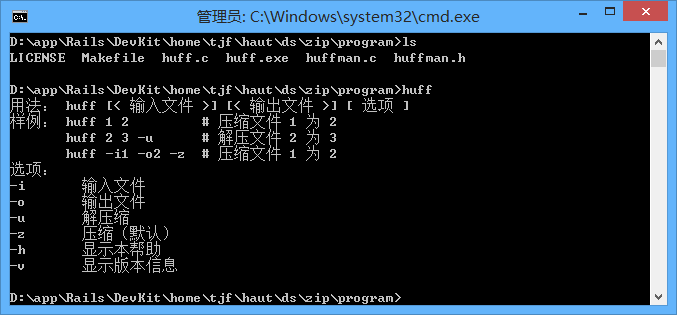
\includegraphics[width=\textwidth]{image/win_huff.png}
\caption{\label{win_huff}}
\end{figure}

如图 \ref{win_test}。我们尝试把编写的源代码文件 {\sf huffman.c} 压缩成 {\sf huffman.c.hf} ,然后把 {\sf huffman.c.hf} 解压成 {\sf huffman.c.rs} 。将原来的 {\sf huffman.c} 和 {\sf huffman.c.rs} 进行比较,发现没有差异,说明压缩算法没有发生数据损失。查看一下文件大小,发现压缩文件的体积确实变小了。这里,9.8K 的源文件压缩成了 7.3K 的压缩文件。

\begin{figure}[htp]
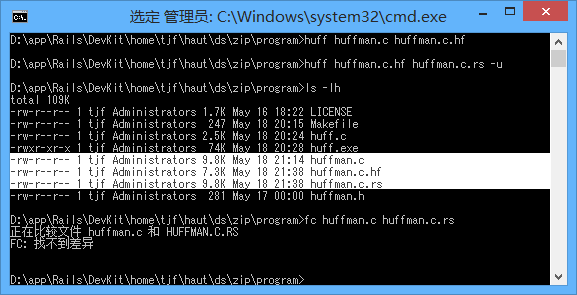
\includegraphics[width=\textwidth]{image/win_test.png}
\caption{\label{win_test}}
\end{figure}

接着我们在 Linux 下进行测试。这里我使用 Putty 以 SSH 连接到虚拟机中的操作系统,执行我需要的命令。图 \ref{linux_huff} 显示了键入程序路径 \verb|./huff| 显示的帮助信息,我们的程序正确地输出了提示信息。

\begin{figure}[htp]
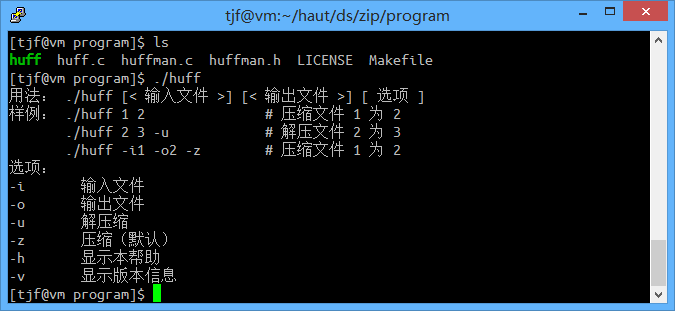
\includegraphics[width=\textwidth]{image/linux_huff.png}
\caption{\label{linux_huff}}
\end{figure}

如图 \ref{linux_test},做相同的测试。由于操作系统存储方式的差异,文件大小有点不一样。但是算法依然是正确的,程序依然产生了正确的输出。

\begin{figure}[htp]
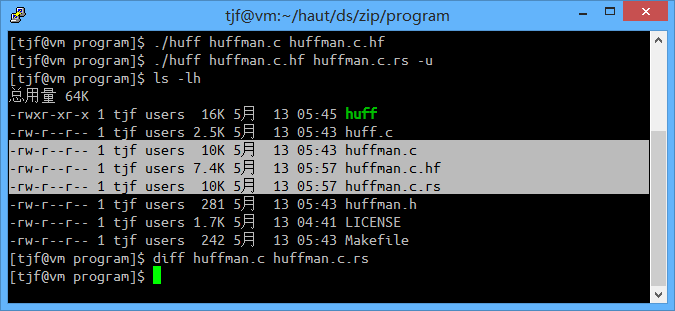
\includegraphics[width=\textwidth]{image/linux_test.png}
\caption{\label{linux_test}}
\end{figure}

可以看到,我们的程序实现了预定目标,工作良好。
